\begin{fullwidth}
    \section{Governance in the Cosmos} \label{sec:governance}

    \begin{adjustwidth}{2cm}{2cm}
        \justify
        The final section of this report focuses on the governance process itself. dYdX Chain governance controls several parameters and processes on dYdX Chain via governance proposals. These proposals may upgrade the Chain's validator software, update parameters, spend the community's resources, and more. In this Section, we briefly describe the governance process on dYdX Chain, including its key parameters. We then overview dYdX's existing governance structures, including the dYdX Grants Program and the dYdX Operations Trust. Finally, we discuss the success of the endorsed delegate program on dYdX v3 and how it may be implemented on dYdX Chain with a less-known CosmosSDK module called \texttt{x/authz}.
    \end{adjustwidth}
    
    \textcolor{gray}{\rule{\linewidth}{0.1mm}}
\end{fullwidth}

    Governance on Cosmos chains has a number of differences and similarities with governance on Ethereum-based protocols. One of the main differences is that votes on Cosmos chains are often cast by the chain's validators. This has been a point of contention for many Cosmos chains, with some arguing that validators should largely abstain from governance and focus on doing what they do best: validating the chain. Governance should instead be conducted by community members with deep domain specific knowledge of the chain, its ecosystem, and priorities. Delegating votes to these community members has become a popular practice amongst many Ethereum-based protocols including dYdX. 

    However, enabling delegation to non-validators poses a technical challenge on Cosmos, which we will discuss. For a great introduction to Cosmos and Cosmos governance purpose-written for dYdX, refer to \bhref{https://dydx.forum/t/dydx-v4-a-beginners-guide-to-cosmos/761}{this} post by RoboMcGobo, a dYdX and Osmosis community member and grantor for the dYdX Grants program. For a more detailed overview of the dYdX Chain governance process, see this comprehensive \href{https://drive.google.com/file/d/1smL9EMRItWbloTJ9u0sxiynKDVvsBH6e/view}{report} from Flipside Crypto's governance team!

    \subsection{The Governance Process}

        \begin{figure}[htp]
            \centering
            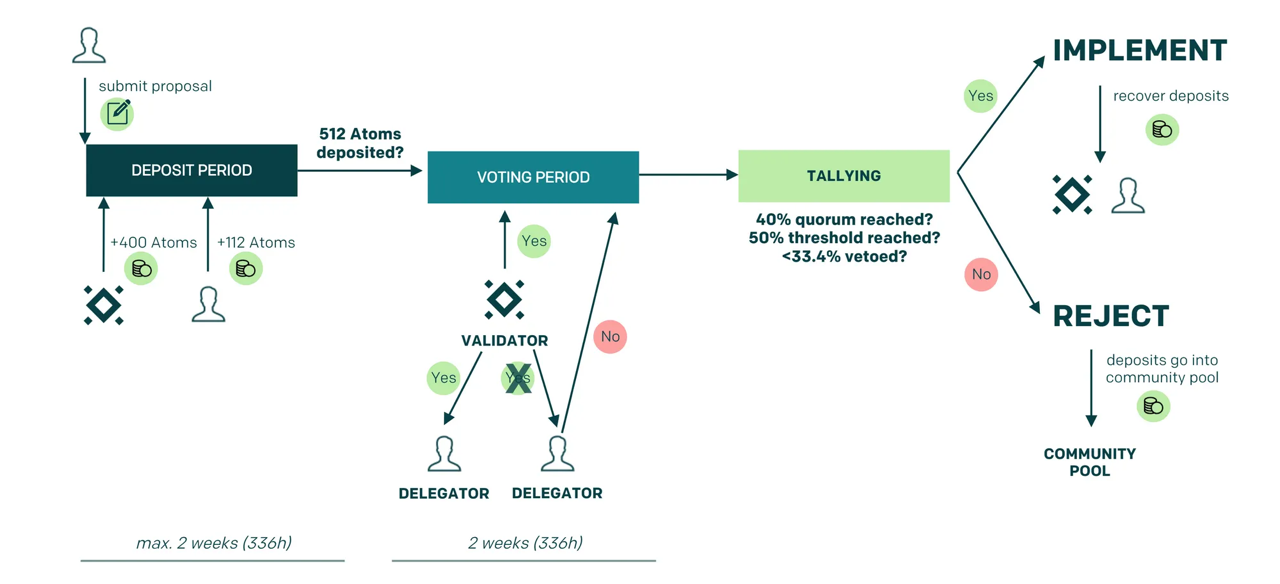
\includegraphics[width=\linewidth]{figs/cosmos_gov.png}
            \caption{The Cosmos governance process, taken from \bhref{https://medium.com/chorus-one/an-overview-of-cosmos-hub-governance-b2b674c2664e}{this} blog post by Felix Lutsch, Chorus One.}
            \label{fig:cosmos_gov}
        \end{figure}

        The CosmosSDK module \texttt{x/gov} underpins the governance process of most Cosmos blockchains, including dYdX Chain. To understand dYdX Chain governance, one must first have a basic understanding of the \texttt{x/gov} process.

        On dYdX Chain any user can submit a proposal along with an initial deposit. The minimum initial deposit required to submit a proposal is defined by the \texttt{min\_initial\_deposit\_ratio} parameter, which can be set to $0$. By raising the minimum initial deposit, governance could throttle the quantity of submissions. This might be appropriate, for example, if the governance process is being overwhelmed by numerous frivolous proposals.

        Following the initial proposal, other token holders might contribute to a proposals initial deposit until a \texttt{min\_deposit} is reached, currently set at $1M$ DYDX as of the latest testnet, which is subject to change. Again, governance may choose to raise or lower this minimum deposit depending on how difficult it is to reach it.

        Once a proposal has reached the minimum deposit, it enters a voting period lasting 7 days. Validators and stakers may vote on a proposal with their staked DYDX. A staker will inherit the vote of their validator unless they choose to manually override it. As it stands, stakers cannot choose to delegate their voting power to any user other than a validator.

        Once the voting period ends, the module will check whether at least $33.4\%$ of staked tokens have voted, known as quorum. If quorum was met, a proposal is implemented as long as more than $50\%$ of votes were in favor of the proposal, and less than $33.4\%$ of votes vetoed the proposal. All these thresholds are parameters than governance may modify through parameter change proposals as well.

        The governance process for the Cosmos Hub is depicted in Fig. \ref{fig:cosmos_gov}, taken from a blog post by Felix Lutsch as Chorus One. Although some governance parameters for the Cosmos Hub are different than those for dYdX Chain, the process is still the same.

        \subsubsection{Relevant Governance Parameters}

            Following the methodology in Appendix \ref{app:genesis}, we reproduce the dYdX Chain testnet governance parameters in Table \ref{tab:x_gov_params}. A key responsibility for dYdX Chain governance will be to the monitor governance process and ensure a fair, transparent process for surfacing important proposals, while minimizing clutter and governance overhead. Part of that responsibility involves tuning and managing these governance parameters, if necessary.

            \begin{table}[htp]
                \centering
                \captionsetup{justification=centering}
                \caption{\texttt{x/gov} Parameters}
                \begin{tabular}{lr}
                    \toprule
                    Name & Value \\
                    \midrule
                    burn\_proposal\_deposit\_prevote & False \\
                    burn\_vote\_quorum & False \\
                    burn\_vote\_veto & True \\
                    max\_deposit\_period & 86400s \\
                    min\_deposit & 1000000 \\
                    min\_initial\_deposit\_ratio & 0 \\
                    quorum & 0.33400 \\
                    threshold & 0.50000 \\
                    veto\_threshold & 0.33400 \\
                    voting\_period & 86400s \\
                    \bottomrule
                \end{tabular}
                \label{tab:x_gov_params}
            \end{table}
        
    \subsection{subDAOs} \label{subsec:subDAOs}

        \sidenotequote{In conclusion, it is claimed that the effective Organization will favor some sort of configuration—some type of a logically consistent clustering of its elements—as it searches for harmony in its internal processes and consonance with its environment.}{\bhref{https://pubsonline.informs.org/doi/10.1287/mnsc.26.3.322}{\textit{Structure in 5's: A Synthesis of the Research on Organization Design}} by Henry Mintzberg}Throughout this report we have discussed the several responsibilities of dYdX governance, or the DAO, in operating dYdX Chain. This includes proposals to spend DYDX on various initiatives, funding grants, slashing misbehaving validators, tuning risk parameters, minimizing fraud in front ends, and much more. Of course, each of these responsibilities requires sophisticated domain-specific knowledge to be adjudicated appropriately. This creates a problem: the DAO has too much responsibility spread amongst individuals who might have competencies in some areas, but not in others. To make the DAO more efficient, we would ideally focus specific decisions on smaller groups of community members and service providers that are particularly knowledgeable about those kinds of decisions! subDAOs, or working groups, are exactly that; subsets of the DAO that have domain specific knowledge that accelerates and improves decision making under a specified mandate.

        dYdX has two primary subDAOs: \bhref{https://dydxopsdao.com/}{the Operations subDAO}, which is led by the dYdX Operations Trust, and \bhref{https://www.dydxgrants.com/}{dYdX Grants}.\sidenotequote{The dYdX Operations subDAO serves the dYdX community, with the mandate to establish a team to set up and operate infrastructure for dYdX v4, the community, and help grow the dYdX ecosystem.}{\bhref{https://dydxopsdao.com/}{dYdX Ops subDAO}}Both subDAOs have clear and distinct mandates to grow and operate the dYdX ecosystem, including and especially its transition to dYdX v4. The grants program primarily manages dYdX's grants budget, vetting and funding teams that contribute to the dYdX ecosystem, as well as providing assistance to grants recipients to accelerate project completion. To date, the dYdX Grants program has facilitated over 120 grants and over \$4M USD of funding across a wide variety of topics.
        
        The purpose of the Ops subDAO is two-fold, part technical and part governance. The technical mandate for the Ops subDAO is to maintain key infrastructure for dYdX Chain, including the chain's three front ends, as well as supporting an external team to maintain one of the chain's indexers. In terms of governance, the Ops subDAO is tasked with helping grow dYdX's ecosystem, including establishing new relevant subDAOs for dYdX Chain. But what subDAOs might be most relevant following the launch of dYdX Chain? 

        \subsubsection{New subDAOs}

            Part of the Ops subDAO's mandate was developing the subDAO \bhref{https://dydx-dao-playbook.webflow.io/post/introduction}{playbook}. Let's take a page of the subDAO playbook to answer the question: when is a subDAO needed?
    
            \begin{displayquote}
                When deciding if a subDAO is needed, we recommend that the Community ask itself: is there a job to be done/information to be found that requires specialization and rapid decision-making? 
    
                If the answer is “yes,” a subDAO could be the answer.
            \end{displayquote}
    
            \begin{marginfigure}
                \centering
                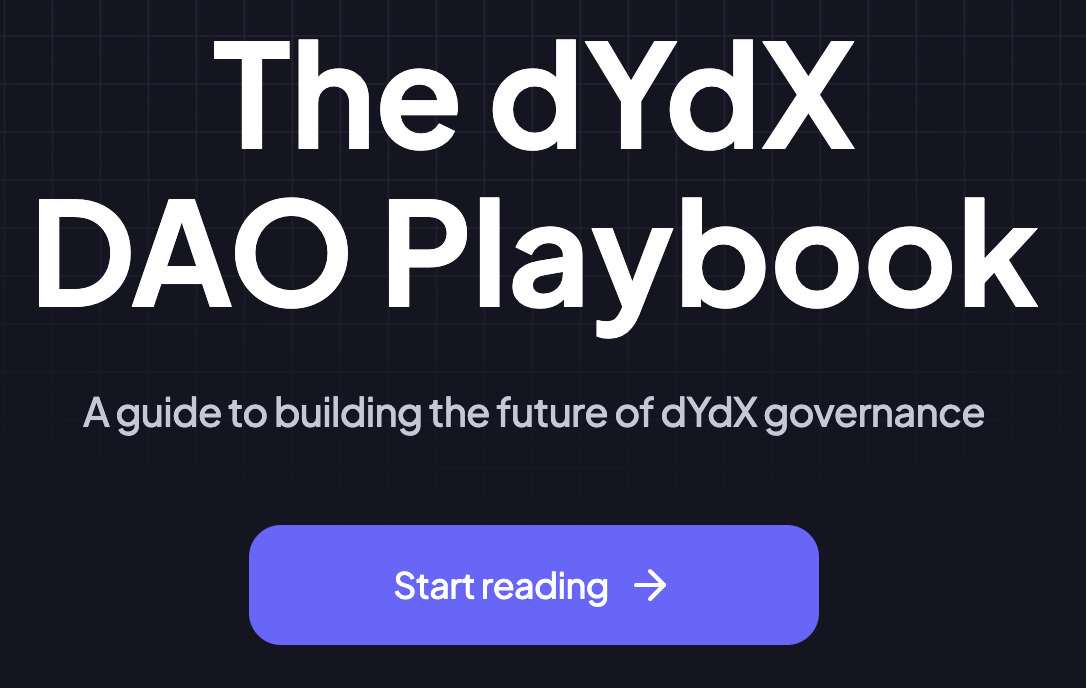
\includegraphics[width=\linewidth]{figs/playbook.png}
                \caption{Screenshot of the Ops subDAO \bhref{https://dydx-dao-playbook.webflow.io/}{playbook}.}
                \label{fig:playbook}
            \end{marginfigure}
    
            Throughout this report, we have touched upon a few key responsibilities for dYdX governance that might be facilitated with either subDAOs or service providers. These have included: risk management of market and liquidation parameters, managing incentives program parameters and expenses, and keeping validators properly incentivized (including reviewing MEV activity). We discuss these and other keys functions within dYdX in Table \ref{tab:subDAOs}\sidenote{Two of these subDAOs are inspired by a \bhref{https://dydx.forum/t/crafting-dydxs-decentralised-future-essential-subdaos-for-consideration/215}{post} from Kagan at Fox Labs (now Cypher Labs), a dYdX community member.}
    
            We test each of these 5 subDAOs against the litmus test from the subDAO playbook in Table \ref{tab:subDAOs}. Notice that many responsibilities overlap between subDAOs, for example: should an Incentives subDAO or a validator management subDAO handle trading fees? In practice, a small subset of these potential subDAOs, such as the Risk subDAO and the Incentives subDAO, could absorb all the high priority responsibilities. Treasury management, for example, could have the operational role of conducting transactions absorbed by the Ops subDAO, whereas the accounting functionality could be offloaded to a service provider or grantee. Monitoring MEV might fall under the mandate of Risk, while ensuring proper validator and market maker incentives might be a task for the Incentives subDAO. Over time, dYdX will identify the minimum viable set of subDAOs to operate efficiently, avoiding the bureaucracy of creating too many overlapping or unnecessary subDAOs, but ensuring key functions can be executed efficiently. If one subDAO has too much on its place, a new subDAO might be formed to partition the original mandate.
    
            \begin{table*}[htp]
                \small
                \centering
                \captionsetup{justification=centering, font=large}
                \caption{dYdX subDAOs - A Litmus Test}
                \begin{tabular}{p{0.1\linewidth} || p{0.18\linewidth} p{0.1\linewidth} p{0.18\linewidth} p{0.1\linewidth} p{0.18\linewidth}}
                    \toprule
                    \textbf{subDAO} & \textbf{Goal} & \textbf{Requires Domain-Specific Knowledge} & \textbf{What Knowledge?} & \textbf{Requires Speedy Decision Making} & \textbf{When?} \\
                    \midrule
                    Risk subDAO & Optimize market risk parameters and prevent unnecessary losses from [missed] liquidations. Maybe: handle asset listings. & Yes & Market and liquidity risk modeling. & Yes & During periods of high market volatility and risk. \\
                    \hline
                    Incentives subDAO & Optimize the protocol's incentives, including Trading Rewards, maker and taker fees/rebates, launch incentives, etc. & Yes & Some behavioral economics; keen understanding of pricing and elasticity. & Unlikely & Decisions with respect to rewards or trading fees are unlikely to require speedy decision making. \\
                    \hline
                    Validator management subDAO & Monitor validator behavior and ensure proper validator incentives & Yes & Knowledge of MEV and the validator business model. & Yes & Catching and punishing MEV quickly could save users significant capital. \\
                    \hline
                    Treasury management subDAO & Conduct transactions from and to community-owned accounts on dYdX Chain, and perform accounting on treasuries. & Some & Some knowledge of transactions on dYdX Chain, and accounting. & Yes & Urgent proposals to consume treasury resources, such as providing emergency capital to the liquidation fund. \\
                    \hline 
                    Business Development subDAO & Manage relationships and service requests from validators, market makers, and other key ecosystem players. & Some & Ideally, members would have deep personal networks with relevant players, and are able to both understand their problems and negotiate reasonable solutions. & Yes & Validators and market makers might have several urgent requests and concerns, many of these might be technical.\\
                    \bottomrule
                \end{tabular}
                \label{tab:subDAOs}
            \end{table*}

    \subsection{Endorsed Delegates}

        The subDAO debate revolves around focusing the right people on the highest priority problems for dYdX, and making it easy for them to operate efficiently. A related component of this process is endorsed delegation. Endorsed delegation allows token holders (or stakers) to delegate their voting power to any user of their choice, instead of exclusively delegating to the chain's validators. In theory, this ``representative democracy'' approach providers token holders with the peace of mind that their tokens are being in their best interest, as each token holder can choose an endorsed delegate that closely aligns with their values and beliefs. 

        On the surface level, it appears that delegating to validators achieves the same effect: one must simply identify a validator that aligns with one's interests as a staker and trader on dYdX Chain. However, to understand why endorsed delegates are an important debate for many existing Cosmos chains, we must understand the potential pitfalls of letting validators vote on behalf of stakers:

        \begin{itemize}
            \item Validators are experts at maintaining high-fidelity systems. They are not necessarily experts on protocol governance, trading incentives, market risk, and the many other aspects of operating a decentralized exchange\sidenote{Some validators, of course, do support robust governance research and operations within their businesses. The governance-competent validators could retain their delegated voting power by also being endorsed delegates on dYdX.}.
            \item Validators have little incentive to participate in governance outside of their reputation. Although some stakers might decide who to stake to based on governance participation, many others simply choose the most profitable validator with the lowest commission rate. Hearkening back to the previous point, a validator's primary competence and primary incentive is being a good system operator.
            \item Validators might have conflicts of interest with other chains. For example, if validator $A$ supports chain $xyz.com$, then they might be incentivized to vote in favor of listing $XYZ$ token on dYdX, regardless of the potential risks associated with $XYZ$ token.
        \end{itemize}

        The endorsed delegate versus validator governance model debate is really a manifestation of the \bhref{https://en.wikipedia.org/wiki/Principal\%E2\%80\%93agent_problem}{Principal-Agent problem}. Ideally, delegators would delegate their voting power to the delegate that best represents their interests. By enabling more than just validators to receive delegated voting power, we would open up the ``delegation marketplace'' to any user. This, in turn, creates a competitive dynamic for delegates to research and identify relevant interest groups that they can represent within the dYdX governance system, and gives delegators more options from which to choose. A larger more competitive marketplace would, some argue, create greater alignment between delegates and delegators. Simultaneously, validators would no longer be expected to participate in the governance process (although they could, and many might choose to), freeing them to focus on their actual business: running a profitable validator node. 

        \begin{marginfigure}
            \centering
            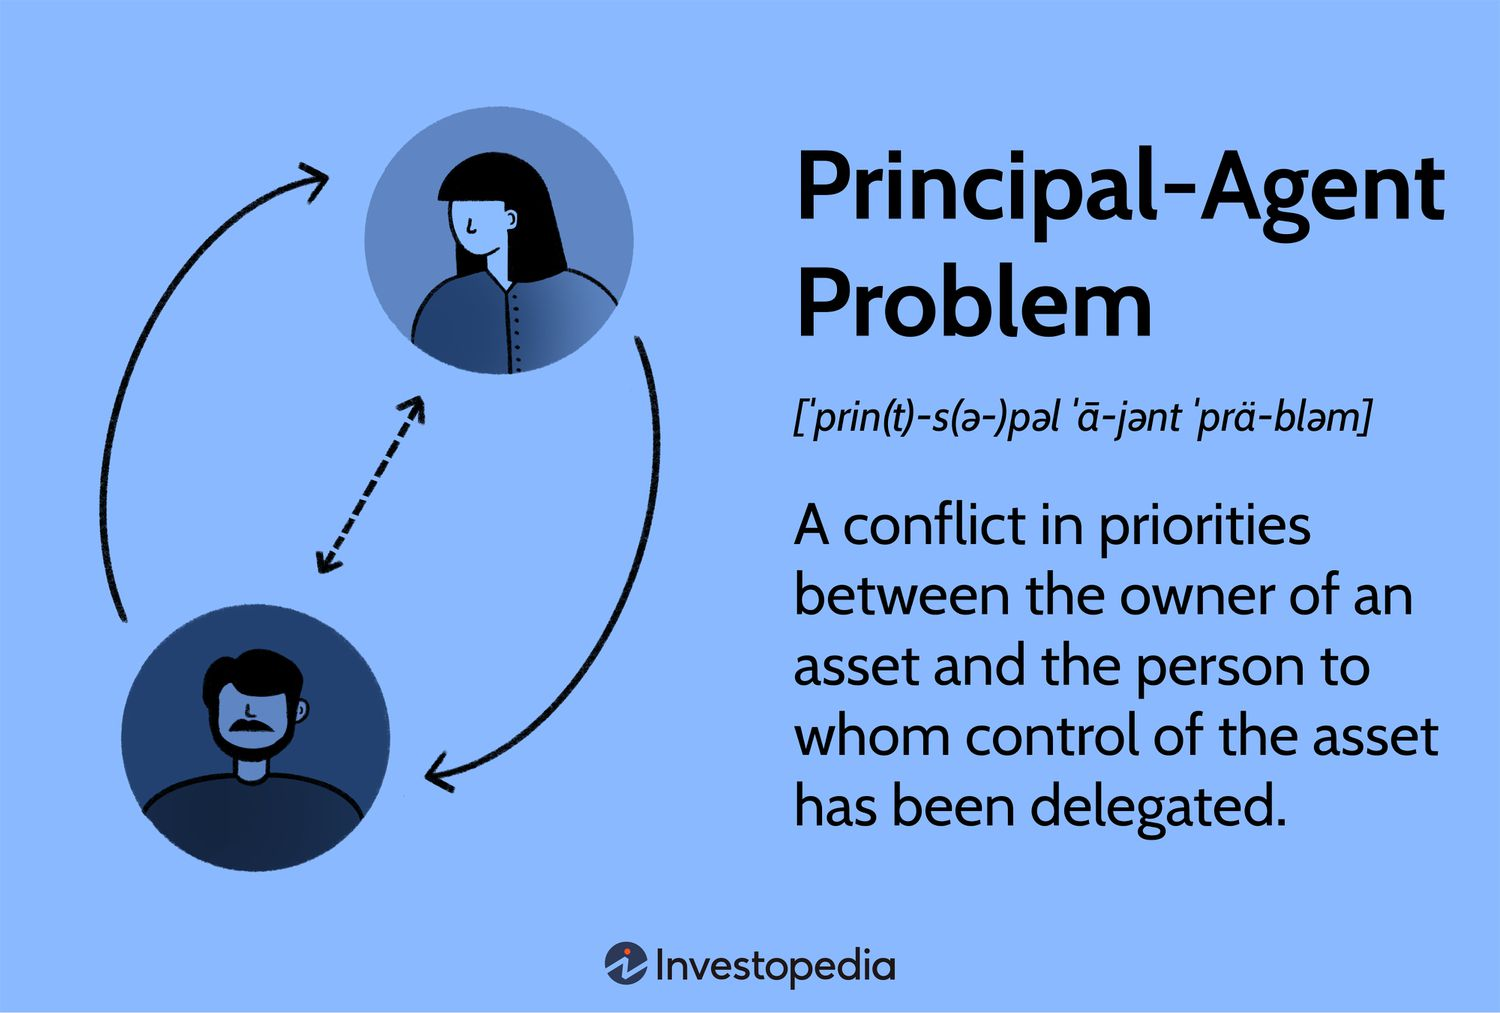
\includegraphics[width=\linewidth]{figs/principal_agent.jpg}
            \caption{The Principal-Agent problem, from \bhref{https://www.investopedia.com/terms/p/principal-agent-problem.asp}{investopedia}.}
            \label{fig:enter-label}
        \end{marginfigure}

        \subsubsection{Endorsed Delegates via \texttt{x/authz}}

            As it stands, endorsed delegation is not implemented on dYdX Chain. This is largely due to a technical challenge of separating the economic value of DYDX tokens with their voting power. That is, a staked DYDX token is escrowed with the validator and can be slashed as well as accrue rewards. This is its economic value. Simultaneously, that same DYDX token holds governance rights, and those governance are delegated to a separate account.

            There is one Cosmos SDK module that enables this kind of separation, the \texttt{x/authz} module. \texttt{x/authz} enables one account to grant arbitrary privileges to another account. Specifically, the module empowers a user (the grantor) to grant another user (the grantee) with the right to submit \texttt{Msg}s on the grantor's behalf. A \texttt{Msg} is a primitive object in any Cosmos chain that defines how the chain transitions from one state to another (recall that a blockchain is really just a machine that computes state transitions). One such \texttt{Msg} might be a \texttt{VoteMsg}, meaning that a user has cast a vote on a particular proposal. Through \texttt{x/authz}, a user might allow another user to submit \texttt{VoteMsg}s on their behalf, thus enabling the process of endorsed delegation.

            Of course, this is a slight oversimplification. For example, there is no canonical user interface for interacting with the \texttt{x/authz} module on any Cosmos chain, although there are some primers and tools for doing so like \bhref{https://github.com/vitwit/resolute/blob/master/HOW_TO.md\#how-to-use-authz-from-resolute-tool}{this} tool from the Resolute team. Furthermore, dYdX Chain will not be implementing the \texttt{x/authz} module at launch, so it must be added and configured at some later point in time.

            Generally, the authors are excited to see \texttt{x/authz} or other superior solutions implemented on dYdX Chain, so that the true underlying market forces of governance can work their magic.